\documentclass[12pt,]{article}
\usepackage{lmodern}
\usepackage{amssymb,amsmath}
\usepackage{ifxetex,ifluatex}
\usepackage{fixltx2e} % provides \textsubscript
\ifnum 0\ifxetex 1\fi\ifluatex 1\fi=0 % if pdftex
  \usepackage[T1]{fontenc}
  \usepackage[utf8]{inputenc}
\else % if luatex or xelatex
  \ifxetex
    \usepackage{mathspec}
  \else
    \usepackage{fontspec}
  \fi
  \defaultfontfeatures{Ligatures=TeX,Scale=MatchLowercase}
\fi
% use upquote if available, for straight quotes in verbatim environments
\IfFileExists{upquote.sty}{\usepackage{upquote}}{}
% use microtype if available
\IfFileExists{microtype.sty}{%
\usepackage{microtype}
\UseMicrotypeSet[protrusion]{basicmath} % disable protrusion for tt fonts
}{}
\usepackage[margin=1.0in]{geometry}
\usepackage{hyperref}
\hypersetup{unicode=true,
            pdftitle={Selective DNA and Protein Isolation from Marine Macrophyte Surfaces},
            pdfborder={0 0 0},
            breaklinks=true}
\urlstyle{same}  % don't use monospace font for urls
\usepackage{graphicx,grffile}
\makeatletter
\def\maxwidth{\ifdim\Gin@nat@width>\linewidth\linewidth\else\Gin@nat@width\fi}
\def\maxheight{\ifdim\Gin@nat@height>\textheight\textheight\else\Gin@nat@height\fi}
\makeatother
% Scale images if necessary, so that they will not overflow the page
% margins by default, and it is still possible to overwrite the defaults
% using explicit options in \includegraphics[width, height, ...]{}
\setkeys{Gin}{width=\maxwidth,height=\maxheight,keepaspectratio}
\IfFileExists{parskip.sty}{%
\usepackage{parskip}
}{% else
\setlength{\parindent}{0pt}
\setlength{\parskip}{6pt plus 2pt minus 1pt}
}
\setlength{\emergencystretch}{3em}  % prevent overfull lines
\providecommand{\tightlist}{%
  \setlength{\itemsep}{0pt}\setlength{\parskip}{0pt}}
\setcounter{secnumdepth}{0}
% Redefines (sub)paragraphs to behave more like sections
\ifx\paragraph\undefined\else
\let\oldparagraph\paragraph
\renewcommand{\paragraph}[1]{\oldparagraph{#1}\mbox{}}
\fi
\ifx\subparagraph\undefined\else
\let\oldsubparagraph\subparagraph
\renewcommand{\subparagraph}[1]{\oldsubparagraph{#1}\mbox{}}
\fi

%%% Use protect on footnotes to avoid problems with footnotes in titles
\let\rmarkdownfootnote\footnote%
\def\footnote{\protect\rmarkdownfootnote}

%%% Change title format to be more compact
\usepackage{titling}

% Create subtitle command for use in maketitle
\providecommand{\subtitle}[1]{
  \posttitle{
    \begin{center}\large#1\end{center}
    }
}

\setlength{\droptitle}{-2em}

  \title{\textbf{Selective DNA and Protein Isolation from Marine Macrophyte
Surfaces}}
    \pretitle{\vspace{\droptitle}\centering\huge}
  \posttitle{\par}
    \author{}
    \preauthor{}\postauthor{}
    \date{}
    \predate{}\postdate{}
  
\usepackage{times} % Times New Roman font
\usepackage[T1]{fontenc}

\usepackage[none]{hyphenat}

\usepackage{setspace}
\doublespacing
\setlength{\parskip}{1em}

\usepackage{lineno}

\usepackage{pdfpages}

\usepackage{indentfirst}

\usepackage[labelsep=period, labelfont=bf]{caption}
\renewcommand{\thefigure}{\arabic{figure}}
\captionsetup{justification=raggedright,singlelinecheck=false}

\usepackage{pdflscape}
\newcommand{\blandscape}{\begin{landscape}}
\newcommand{\elandscape}{\end{landscape}}

\usepackage{siunitx}
\DeclareSIUnit\molar{\mole\per\cubic\deci\metre}
\DeclareSIUnit\Molar{\textsc{m}}

\begin{document}
\maketitle

\vspace{80mm}

\textsuperscript{1\(\dagger\)}

\vspace{40mm}

\(\dagger\) To whom correspondence should be addressed:
\href{mailto:marino.korlevic@irb.hr}{\nolinkurl{marino.korlevic@irb.hr}}

1. Ruđer Bošković Institute, Center for Marine Research, G. Paliaga 5,
Rovinj, Croatia

2. University of Vienna, Department of Limnology and Bio-Oceanography,
Althanstraße 14, Vienna, Austria \newpage
\linenumbers
\sisetup{mode=text} \setlength\parindent{24pt}

\subsection{Abstract}\label{abstract}

\newpage

\subsection{Introduction}\label{introduction}

Surfaces of marine macrophytes are inhabited by a diverse microbial
community whose structure and function are poorly understood (Egan
\emph{et al.}, 2013). As less than 1 \% of all prokaryotic species are
culturable, to study these organisms, molecular methods such as 16S rRNA
sequencing, metagenomics and metaproteomics are indispensable (Amann
\emph{et al.}, 1995; Su \emph{et al.}, 2012). Applying these techniques
requires an initial isolation step, with the purpose of obtaining high
quality DNA and proteins.

Biological material (i.e.~proteins and DNA) from pelagic microbial
communities is usually isolated by collecting cells onto filters and
subsequently isolating the aimed compound (Gilbert \emph{et al.}, 2009).
If a microbial size fraction is aimed sequential filtration is applied
(Massana \emph{et al.}, 1997; Andersson \emph{et al.}, 2010). In
contrast, obtaining biological materials from microorganism inhabiting
surfaces requires either a cell detachment procedure prior to isolation
or the host material is coextracted together with the targeted material.
Methods for separating microbial cells form the host include shaking of
host tissue (Gross \emph{et al.}, 2003; Nõges \emph{et al.}, 2010),
scraping of macrophyte surfaces (Uku \emph{et al.}, 2007) or the
application of ultrasonication (Weidner \emph{et al.}, 1996; Cai
\emph{et al.}, 2014). It was shown that shaking alone is not sufficient
to remove microbial cells, at least from plant root surfaces
(Richter-Heitmann \emph{et al.}, 2016). Manual separation methods, such
as scraping and brushing, are time consuming and subjective, as the
detachment efficiency depends on host tissue and the person performing
the procedure (Cai \emph{et al.}, 2014). Ultrasonication was proposed as
an alternative method as it is providing better results in terms of
detachment efficiency (Cai \emph{et al.}, 2014; Richter-Heitmann
\emph{et al.}, 2016). The downside of this procedure is that complete
cell removal was still not obtained and tissue disruption was observed
especially after the application of probe ultrasonication
(Richter-Heitmann \emph{et al.}, 2016). An alternative to these cell
detachment procedures is the isolation of targeted epiphytic compounds
together with host materials (Staufenberger \emph{et al.}, 2008; Jiang
\emph{et al.}, 2015). This procedure can lead to problems in the
following processing steps such as mitochondrial and chloroplast 16S
rRNA sequence contaminations from the host (Longford \emph{et al.},
2007; Staufenberger \emph{et al.}, 2008). In addition, when performing
metagenomics and metaproteomics host material can cause biased results
towards more abundant host DNA and proteins.

An alternative to these procedures is a direct isolation of the targeted
material by incubating macrophyte tissues in an extraction buffer. After
the incubation is done the undisrupted host tissue is removed and the
isolation procedure continues omitting host material contaminations. To
our knowledge the only procedure describing a direct and selective
epiphytic DNA isolation from the surfaces of marine macrophytes was
provided by Burke \emph{et al.} (2009). In contrast to previously
described methods this protocol enables an almost complete removal of
the surface community and was used for 16S rRNA gene clone libraries
construction (Burke \emph{et al.}, 2011b) and metagenomes sequencing
(Burke \emph{et al.}, 2011a). This method, thought providing a selective
isolation procedure, is using in the extraction buffer a rapid
multienzyme cleaner (3M) that is not worldwide available and whose
composition is not know (Burke \emph{et al.}, 2009). Also to our
knowledge, no selective isolation protocol for proteins from epiphytic
communities inhabiting marine macrophytes was established.

In the present study, we adapted a protocol widely used for DNA
isolation from filters (Massana \emph{et al.}, 1997) and a protocol used
for protein isolation from sediments (Chourey \emph{et al.}, 2010;
Hultman \emph{et al.}, 2015) for selective extractions of DNA and
proteins from epiphytic communities inhabiting the surfaces of two
marine macrophytes: the seagrass \emph{Cymodocea nodosa} and the alga
\emph{Caulerpa cylindracea}. In addition, we tested the removal
efficiency of the protocol and the suitability of obtained DNA and
proteins for 16S rRNA sequencing and metaproteomics.

\newpage

\subsection{Materials and Methods}\label{materials-and-methods}

\subsubsection{Sampling}\label{sampling}

Leaves of \emph{Cymodocea nodosa} were sampled in a \emph{Cymodocea
nodosa} meadow in the Bay of Saline (45°7´5˝N, 13°37´20˝E) and in a
\emph{Cymodocea nodosa} meadow invaded by \emph{Caulerpa cylindracea} in
the proximity of the village of Funtana (45°10´39˝N, 13°35´42˝E). Thalli
of \emph{Caulerpa cylindracea} were sampled in the same \emph{Cymodocea
nodosa} invaded meadow in Funtana and on a locality of only
\emph{Caulerpa cylindracea} located in the proximity of the invaded
meadow. Leaves and thalli were collected on the same day in two
contrasting seasons, on 4 December 2017 and 18 June 2018. During spring
2018 the \emph{Cymodocea nodosa} meadow in the Bay of Saline decayed to
an extent that no leaves could be retrieved (Najdek \emph{et al.},
unpublished data). Leaves and thalli were collected by diving and
transported to the laboratory in containers placed on ice and filled
with site seawater. Upon arrival to the laboratory, \emph{Cymodocea
nodosa} leaves were cut into sections of 1 -- 2 \si{\cm}, while
\emph{Caulerpa cylindracea} thalli were cut into 5 -- 8 \si{\cm} long
sections. Leaves and thalli were washed three times with sterile
artificial seawater (ASW) to remove loosely attached microbial cells.

\subsubsection{DNA Isolation}\label{dna-isolation}

The DNA was isolated according to the protocol for isolation from
filters described in Massana \emph{et al.} (1997). This protocol was
modified and adapted for DNA isolation from microbial communities from
macrophyte surfaces as described below. 5 \si{\ml} of lysis buffer (40
\si{\milli\Molar} EDTA, 50 \si{\milli\Molar} Tris-HCl, 0.75 \si{\Molar}
sucrose; pH 8.3) was added to 1 \si{\g} wet weight of leaves or \si{\g}
wet-weight of thalli. Lysozyme was added (final concentration 1
\si{\mg\per\ml}) and the mixture was incubated at 37 \si{\degreeCelsius}
for 30 \si{\minute}. Subsequently, proteinase K (final concentration 0.5
\si{\mg\per\ml}) and SDS (final concentration 1 \si{\percent}) were
added and the samples were incubated at 55 \si{\degreeCelsius} for 2
\si{\hour}. Following the incubation, tubes were vortexed for 10
\si{\minute} and the mixture containing lyzed epiphytic cells was
separated from host leaves or thalli by transferring the solution into a
clean tube. The lysate was extracted twice with a mixture of
phenol:chloroform:isoamyl alcohol (25:24:1; pH 8) and once with
chloroform:isoamyl alcohol (24:1). After each organic solvent mixture
addition tubes were slightly vortexed and centrifuged at 4,500 × g for
10 \si{\minute}. Following each centrifugation aqueous phases were
retrieved. After the final extraction 1/10 of chilled 3 \si{\Molar}
sodium acetate (pH 5.2) was added. DNA was precipitated by adding 1
volume of chilled isopropanol, incubating the mixtures overnight at
\num{-20} °C and centrifuging at 16,000 × g and 4 \si{\degreeCelsius}
for 20 \si{\minute}. The pellet was washed twice with 1 \si{\ml} of
chilled isopropanol and centrifuged after each washing step at 20,000 ×
g and 4 \si{\degreeCelsius} for 10 \si{\minute}. After the first washing
step duplicate pellets form the same sample were pooled and transferred
to a clean 1.5 \si{\ml} tube. The dried pellet was resuspended in 100
\si{\ul} of deionized water.

\subsubsection{Illumina 16S rRNA
Sequencing}\label{illumina-16s-rrna-sequencing}

An aliquot of isolated DNA was treated with RNase A (final concentration
200 \si{\ug\per\ml}) for 2 \si{\hour} at 37 \si{\degreeCelsius}. The DNA
concentration was determined using the Quant-iT PicoGreen dsDNA Assay
Kit (Invitrogen, USA) according to the manufacturer's instructions and
diluted to 1 \si{\ng\per\ul}. The V4 region of the 16S rRNA gene was
amplified using a two-step PCR procedure. In the first PCR the 515F
(5'-GTGYCAGCMGCCGCGGTAA-3') and 806R (5'-GGACTACNVGGGTWTCTAAT-3')
primers from the Earth Microbiome Project
(\url{http://press.igsb.anl.gov/earthmicrobiome/protocols-and-standards/16s/})
were used to amplify the target region (Caporaso \emph{et al.}, 2012;
Apprill \emph{et al.}, 2015; Parada \emph{et al.}, 2016). These primers
contained on their 5' end a tagged sequence. Each sample was amplified
in four parallel 25 \si{\ul} reactions of which each contained: 1 × Q5
Reaction Buffer , 0.2 \si{\milli\Molar} of dNTPmix, 0.7 \si{\mg\per\ml}
BSA (Bovine Serum Albumin), 0.2 \si{\micro\Molar} of forward and reverse
primers, 0.5 U of Q5 High-Fidelity DNA Polymerase (New England Biolabs,
USA) and 5 \si{\ng} of DNA template. Cycling conditions were: initial
denaturation at 94 \si{\degreeCelsius} for 3 \si{\minute}, 20 cycles of
denaturation at 94 \si{\degreeCelsius} for 45 \si{\s}, annealing at 50
\si{\degreeCelsius} for 60 \si{\s} and elongation at 72
\si{\degreeCelsius} for 90 \si{\s}, finalized by an elongation step at
72 \si{\degreeCelsius} for 10 \si{\minute}. The four parallel reactions
volumes were pooled and PCR products were purified using the GeneJET PCR
Purification Kit (Thermo Fisher Scientific, USA) according to the
manufacturer's instructions and following the protocol that included
isopropanol addition for better small DNA fragment yield. The column was
eluted in 30 \si{\ul} of deionized water. Purified PCR products were
sent for Illumina MiSeq sequencing (2 × 250 bp) at IMGM Laboratories,
Martinsried, Germany. Before sequencing, at IMGM the second PCR
amplification of the two-step PCR procedure was performed using primers
targeting the tagged region incorporated in the first PCR. In addition,
these primers contained adapter and sample-specific index sequences. The
second PCR was carried out for 8 cycles. Beside samples, a positive and
negative control were sequenced. A negative control was comprised of
four parallel PCR reactions without DNA template, while for a positive
control a mock community composed of evenly mixed DNA material
originating from 20 bacterial strains (ATCC MSA-1002, ATCC, USA) was
used. The sequences obtained in this study have been submitted to the
European Nucleotide Archive (ENA) under accession numbers \textbf{TO BE
ADDED LATER!}.

\subsubsection{Sequence Analysis}\label{sequence-analysis}

Obtained sequences were analyzed on the computer cluster Isabella
(University Computing Center, University of Zagreb) using mothur
(version 1.43.0) (Schloss \emph{et al.}, 2009) according to the MiSeq
Standard Operating Procedure (MiSeq SOP;
\url{https://mothur.org/wiki/MiSeq_SOP}) (Kozich \emph{et al.}, 2013)
and recommendations given from the Riffomonas project to enhance data
reproducibility (\url{http://www.riffomonas.org/}). For alignment and
classification of sequences the SILVA SSU Ref NR 99 database (release
132; \url{http://www.arb-silva.de}) was used (Quast \emph{et al.}, 2013;
Yilmaz \emph{et al.}, 2014). Sequences classified as chloroplasts by
mothur were exported, aligned using SILVA incremental aligner (SINA,
version 1.6.0) (Pruesse \emph{et al.}, 2012) against the same SILVA SSU
Ref NR 99 database (release 132) and imported into ARB (version 6.0.6)
(Ludwig \emph{et al.}, 2004) for further phylogenetic analysis using the
same database. Reference sequences close to imported ones were selected
and used to calculate a phylogenetic tree using the Maximum Likelihood
algorithm RAxML (version 7.0.3) with 1000 tree replicates (Stamatakis,
2006). Imported partial chloroplast sequences were added to the tree
using the maximum parsimony criteria and not allowing changes to tree
topology. Pipeline data processing and visualization was done using R
(version 3.6.0) (R Core Team, 2019), package tidyverse (version 1.2.1)
(Wickham \emph{et al.}, 2019) and multiple other packages (Xie, 2014,
2015, 2019a, 2019b; Xie \emph{et al.}, 2018; Zhu, 2019; Allaire \emph{et
al.}, 2019). The detailed analysis procedure including the R Markdown
file for this paper are available as a GitHub repository (\textbf{TO BE
ADDED LATER!}). Based on the ATCC MSA-1002 mock community included in
the analysis a sequencing error rate of 0.009 \si{\percent} was
determined, which is in line with previously reported values for
next-generation sequencing data (Kozich \emph{et al.}, 2013; Schloss
\emph{et al.}, 2016). In addition, the negative control processed
together with the samples yielded only 2 sequences after sequence
quality curation.

\subsubsection{Protein Isolation}\label{protein-isolation}

Proteins were isolated according to the protocol for isolation from soil
described in Chourey \emph{et al.} (2010) and modified by Hultman
\emph{et al.} (2015). These protocols were further modified and adapted
for protein isolation from microbial communities form macrophyte
surfaces as described below. 20 \si{\ml} of protein extraction buffer (4
\si{\percent} SDS, 100 \si{\milli\Molar} Tris-HCl {[}pH 8.0{]}) was
added to 5 \si{\g} wet weight of leaves or 10 \si{\g} wet weight of
thalli. The mixture was incubated in boiling water for 5 \si{\minute},
vortexed for 10 \si{\minute} and incubated again in boiling water for 5
\si{\minute}. After a brief vortex the lysate was transferred to a clean
tube separating the host leaves or thalli from the mixture containing
lyzed epiphytic cells. Dithiothreitol (DTT; final concentration 24
\si{\milli\Molar}) was added and proteins were precipitated with chilled
100 \si{\percent} trichloroacetic acid (TCA; final concentration 20
\si{\percent}) overnight at \num{-20} °C. Precipitated proteins were
centrifuged at 10,000 × g and 4 \si{\degreeCelsius} for 40 \si{\minute}.
The obtained protein pellet was washed three times with chilled acetone.
During the first washing step the pellet was transferred to a clean 1.5
\si{\ml} tube. After each washing step samples were centrifuged at
20,000 × g and 4 \si{\degreeCelsius} for 5 \si{\minute}. Dried pellets
were stored at \num{-80} °C until further analysis.

\subsubsection{Metaproteomics}\label{metaproteomics}

Isolated proteins were whole trypsin digested using the FASP
(filter-aided sample preparation) Protein Digestion Kit (Expedeon, UK)
according to the manufacturer's instructions (Wiśniewski \emph{et al.},
2009) with small modifications. Before loading the solution to the
column, protein pellets were solubilized in a urea sample buffer
included in the kit amended with DTT (final concentration 100
\si{\milli\Molar}) for 45 \si{\minute} at room temperature and
centrifuged at 20,000 × g for 2 -- 5 \si{\minute} at room temperature to
remove larger particles. The first washing step after protein solution
loading was repeated twice. In addition, centrifugation steps were
prolonged if the column was clogged. Trypsin digestion was performed on
column filters at 37 \si{\degreeCelsius} overnight for 18 \si{\hour}.
The final filtrate containing digested proteins was acidified with 1
\si{\percent} (final concentration) trifluoroacetic acid, freezed at
\num{-80} \si{\degreeCelsius} for 15 \si{\minute}, lyophilized and sent
to the Vienna Metabolomics Center (University of Vienna) for
metaproteomic analysis. \textbf{TO BE ADDED-VIENNA PART}.

\subsubsection{Confocal Microscopy}\label{confocal-microscopy}

Host leaves and thalli from DNA and protein isolation steps were washed
seven times in deionized water and fixed with formaldehyde (final
concentration \textasciitilde{} 3 \si{\percent}). In addition,
nontreated leaves and thalli, washed three times in ASW to remove
loosely attached microbial cells, were fixed in the same concentration
of formaldehyde and used as a positive control. For long therm storage,
fixed leaves and thalli were immersed in a mixture of phosphate-buffered
saline (PBS) and ethanol (1:1) and stored at \num{-20}
\si{\degreeCelsius}. Treated and untreated leaves and thalli segments
were stained in a 2 × solution of SYBR Green I and examined under a
Leica TCS SP8 X FLIM confocal microscope (Leica Microsystems, Germany).

\subsection{Results}\label{results}

\subsection{Discussion}\label{discussion}

\subsection{Acknowledgements}\label{acknowledgements}

\newpage

\subsection{References}\label{references}

\hypertarget{refs}{}
\hypertarget{ref-Allaire2019}{}
Allaire, J.J., Xie, Y., McPherson, J., Luraschi, J., Ushey, K., Atkins,
A., et al. (2019) rmarkdown: Dynamic Documents for R.

\hypertarget{ref-Amann1995}{}
Amann, R.I., Ludwig, W., and Schleifer, K.H. (1995) Phylogenetic
identification and in situ detection of individual microbial cells
without cultivation. \emph{Microbiological reviews} \textbf{59}:
143--169.

\hypertarget{ref-Andersson2010}{}
Andersson, A.F., Riemann, L., and Bertilsson, S. (2010) Pyrosequencing
reveals contrasting seasonal dynamics of taxa within Baltic Sea
bacterioplankton communities. \emph{The ISME journal} \textbf{4}:
171--181.

\hypertarget{ref-Apprill2015}{}
Apprill, A., McNally, S., Parsons, R., and Weber, L. (2015) Minor
revision to V4 region SSU rRNA 806R gene primer greatly increases
detection of SAR11 bacterioplankton. \emph{Aquatic Microbial Ecology}
\textbf{75}: 129--137.

\hypertarget{ref-Burke2009}{}
Burke, C., Kjelleberg, S., and Thomas, T. (2009) Selective extraction of
bacterial DNA from the surfaces of macroalgae. \emph{Applied and
environmental microbiology} \textbf{75}: 252--256.

\hypertarget{ref-Burke2011a}{}
Burke, C., Steinberg, P., Rusch, D., Kjelleberg, S., and Thomas, T.
(2011a) Bacterial community assembly based on functional genes rather
than species. \emph{Proceedings of the National Academy of Sciences of
the United States of America} \textbf{108}: 14288--14293.

\hypertarget{ref-Burke2011b}{}
Burke, C., Thomas, T., Lewis, M., Steinberg, P., and Kjelleberg, S.
(2011b) Composition, uniqueness and variability of the epiphytic
bacterial community of the green alga Ulva australis. \emph{The ISME
journal} \textbf{5}: 590--600.

\hypertarget{ref-Cai2014}{}
Cai, X., Gao, G., Yang, J., Tang, X., Dai, J., Chen, D., and Song, Y.
(2014) An ultrasonic method for separation of epiphytic microbes from
freshwater submerged macrophytes. \emph{Journal of basic microbiology}
\textbf{54}: 758--761.

\hypertarget{ref-Caporaso2012}{}
Caporaso, J.G., Lauber, C.L., Walters, W.A., Berg-Lyons, D., Huntley,
J., Fierer, N., et al. (2012) Ultra-high-throughput microbial community
analysis on the Illumina HiSeq and MiSeq platforms. \emph{The ISME
Journal} \textbf{6}: 1621--1624.

\hypertarget{ref-Chourey2010}{}
Chourey, K., Jansson, J., VerBerkmoes, N., Shah, M., Chavarria, K.L.,
Tom, L.M., et al. (2010) Direct Cellular Lysis/Protein Extraction
Protocol for Soil Metaproteomics. \emph{Journal of Proteome Research}
\textbf{9}: 6615--6622.

\hypertarget{ref-Egan2013}{}
Egan, S., Harder, T., Burke, C., Steinberg, P., Kjelleberg, S., and
Thomas, T. (2013) The seaweed holobiont: understanding seaweed-bacteria
interactions. \emph{FEMS microbiology reviews} \textbf{37}: 462--476.

\hypertarget{ref-Gilbert2009}{}
Gilbert, J.A., Field, D., Swift, P., Newbold, L., Oliver, A., Smyth, T.,
et al. (2009) The seasonal structure of microbial communities in the
Western English Channel. \emph{Environmental Microbiology} \textbf{11}:
3132--3139.

\hypertarget{ref-Gross2003}{}
Gross, E.M., Feldbaum, C., and Graf, A. (2003) Epiphyte biomass and
elemental composition on submersed macrophytes in shallow eutrophic
lakes. \emph{Hydrobiologia} \textbf{506-509}: 559--565.

\hypertarget{ref-Hultman2015}{}
Hultman, J., Waldrop, M.P., Mackelprang, R., David, M.M., McFarland, J.,
Blazewicz, S.J., et al. (2015) Multi-omics of permafrost, active layer
and thermokarst bog soil microbiomes. \emph{Nature} \textbf{521}:
208--212.

\hypertarget{ref-Jiang2015}{}
Jiang, Y.-F., Ling, J., Dong, J.-D., Chen, B., Zhang, Y.-Y., Zhang,
Y.-Z., and Wang, Y.-S. (2015) Illumina-based analysis the microbial
diversity associated with Thalassia hemprichii in Xincun Bay, South
China Sea. \emph{Ecotoxicology (London, England)} \textbf{24}: 1548--56.

\hypertarget{ref-Kozich2013}{}
Kozich, J.J., Westcott, S.L., Baxter, N.T., Highlander, S.K., and
Schloss, P.D. (2013) Development of a dual-index sequencing strategy and
curation pipeline for analyzing amplicon sequence data on the MiSeq
Illumina sequencing platform. \emph{Applied and environmental
microbiology} \textbf{79}: 5112--5120.

\hypertarget{ref-Longford2007}{}
Longford, S., Tujula, N., Crocetti, G., Holmes, A., Holmström, C.,
Kjelleberg, S., et al. (2007) Comparisons of diversity of bacterial
communities associated with three sessile marine eukaryotes.
\emph{Aquatic Microbial Ecology} \textbf{48}: 217--229.

\hypertarget{ref-Ludwig2004}{}
Ludwig, W., Strunk, O., Westram, R., Richter, L., Meier, H., Yadhukumar,
et al. (2004) ARB: a software environment for sequence data.
\emph{Nucleic Acids Research} \textbf{32}: 1363--1371.

\hypertarget{ref-Massana1997}{}
Massana, R., Murray, A.E., Preston, C.M., and DeLong, E.F. (1997)
Vertical distribution and phylogenetic characterization of marine
planktonic Archaea in the Santa Barbara Channel. \emph{Applied and
environmental microbiology} \textbf{63}: 50--56.

\hypertarget{ref-Noges2010}{}
Nõges, T., Luup, H., and Feldmann, T. (2010) Primary production of
aquatic macrophytes and their epiphytes in two shallow lakes (Peipsi and
Võrtsjärv) in Estonia. \emph{Aquatic Ecology} \textbf{44}: 83--92.

\hypertarget{ref-Parada2016}{}
Parada, A.E., Needham, D.M., and Fuhrman, J.A. (2016) Every base
matters: assessing small subunit rRNA primers for marine microbiomes
with mock communities, time series and global field samples.
\emph{Environmental Microbiology} \textbf{18}: 1403--1414.

\hypertarget{ref-Pruesse2012}{}
Pruesse, E., Peplies, J., and Glöckner, F.O. (2012) SINA: accurate
high-throughput multiple sequence alignment of ribosomal RNA genes.
\emph{Bioinformatics (Oxford, England)} \textbf{28}: 1823--1829.

\hypertarget{ref-Quast2013}{}
Quast, C., Pruesse, E., Yilmaz, P., Gerken, J., Schweer, T., Yarza, P.,
et al. (2013) The SILVA ribosomal RNA gene database project: improved
data processing and web-based tools. \emph{Nucleic acids research}
\textbf{41}: D590--6.

\hypertarget{ref-RCoreTeam2019}{}
R Core Team (2019) R: A Language and Environment for Statistical
Computing, Vienna, Austria: R Foundation for Statistical Computing.

\hypertarget{ref-Richter-Heitmann2016}{}
Richter-Heitmann, T., Eickhorst, T., Knauth, S., Friedrich, M.W., and
Schmidt, H. (2016) Evaluation of Strategies to Separate Root-Associated
Microbial Communities: A Crucial Choice in Rhizobiome Research.
\emph{Frontiers in Microbiology} \textbf{7}: 773.

\hypertarget{ref-Schloss2016}{}
Schloss, P.D., Girard, R.A., Martin, T., Edwards, J., and Thrash, J.C.
(2016) Status of the Archaeal and Bacterial Census: an Update.
\emph{mBio} \textbf{7}: e00201--16.

\hypertarget{ref-Schloss2009}{}
Schloss, P.D., Westcott, S.L., Ryabin, T., Hall, J.R., Hartmann, M.,
Hollister, E.B., et al. (2009) Introducing mothur: open-source,
platform-independent, community-supported software for describing and
comparing microbial communities. \emph{Applied and environmental
microbiology} \textbf{75}: 7537--7541.

\hypertarget{ref-Stamatakis2006}{}
Stamatakis, A. (2006) RAxML-VI-HPC: maximum likelihood-based
phylogenetic analyses with thousands of taxa and mixed models.
\emph{Bioinformatics} \textbf{22}: 2688--2690.

\hypertarget{ref-Staufenberger2008}{}
Staufenberger, T., Thiel, V., Wiese, J., and Imhoff, J.F. (2008)
Phylogenetic analysis of bacteria associated with Laminaria saccharina.
\emph{FEMS Microbiology Ecology} \textbf{64}: 65--77.

\hypertarget{ref-Su2012}{}
Su, C., Lei, L., Duan, Y., Zhang, K.-Q., and Yang, J. (2012)
Culture-independent methods for studying environmental microorganisms:
methods, application, and perspective. \emph{Applied microbiology and
biotechnology} \textbf{93}: 993--1003.

\hypertarget{ref-Uku2007}{}
Uku, J., Björk, M., Bergman, B., and Díez, B. (2007) Characterization
and comparison of prokaryotic epiphytes associated with three East
African seagrasses. \emph{Journal of Phycology} \textbf{43}: 768--779.

\hypertarget{ref-Weidner1996}{}
Weidner, S., Arnold, W., and Puhler, A. (1996) Diversity of uncultured
microorganisms associated with the seagrass Halophila stipulacea
estimated by restriction fragment length polymorphism analysis of
PCR-amplified 16S rRNA genes. \emph{Applied and environmental
microbiology} \textbf{62}: 766--771.

\hypertarget{ref-Wickham2019}{}
Wickham, H., Averick, M., Bryan, J., Chang, W., McGowan, L.D., François,
R., et al. (2019) Welcome to the tidyverse. \emph{Journal of Open Source
Software} \textbf{4}: 1686.

\hypertarget{ref-Wisniewski2009}{}
Wiśniewski, J.R., Zougman, A., Nagaraj, N., and Mann, M. (2009)
Universal sample preparation method for proteome analysis. \emph{Nature
Methods} \textbf{6}: 359--362.

\hypertarget{ref-Xie2015}{}
Xie, Y. (2015) Dynamic Documents with \{R\} and knitr, 2nd ed. Boca
Raton, Florida: Chapman; Hall/CRC.

\hypertarget{ref-Xie2014}{}
Xie, Y. (2014) knitr: A Comprehensive Tool for Reproducible Research in
\{R\}. In, Stodden,V., Leisch,F., and Peng,R.D. (eds),
\emph{Implementing reproducible computational research}. Chapman;
Hall/CRC.

\hypertarget{ref-Xie2019a}{}
Xie, Y. (2019a) knitr: A General-Purpose Package for Dynamic Report
Generation in R.

\hypertarget{ref-Xie2019}{}
Xie, Y. (2019b) tinytex: Helper Functions to Install and Maintain 'TeX
Live', and Compile 'LaTeX' Documents.

\hypertarget{ref-Xie2018}{}
Xie, Y., Allaire, J.J., and Grolemund, G. (2018) R Markdown: The
Definitive Guide, Boca Raton, Florida: Chapman; Hall/CRC.

\hypertarget{ref-Yilmaz2014}{}
Yilmaz, P., Parfrey, L.W., Yarza, P., Gerken, J., Pruesse, E., Quast,
C., et al. (2014) The SILVA and ``All-species Living Tree Project
(LTP)'' taxonomic frameworks. \emph{Nucleic acids research} \textbf{42}:
D643--8.

\hypertarget{ref-Zhu2019}{}
Zhu, H. (2019) kableExtra: Construct Complex Table with 'kable' and Pipe
Syntax.

\newpage 

\subsection{Figure Captions}\label{figure-captions}

\subsection{Figures}\label{figures}

\begin{figure}[h]

{\centering 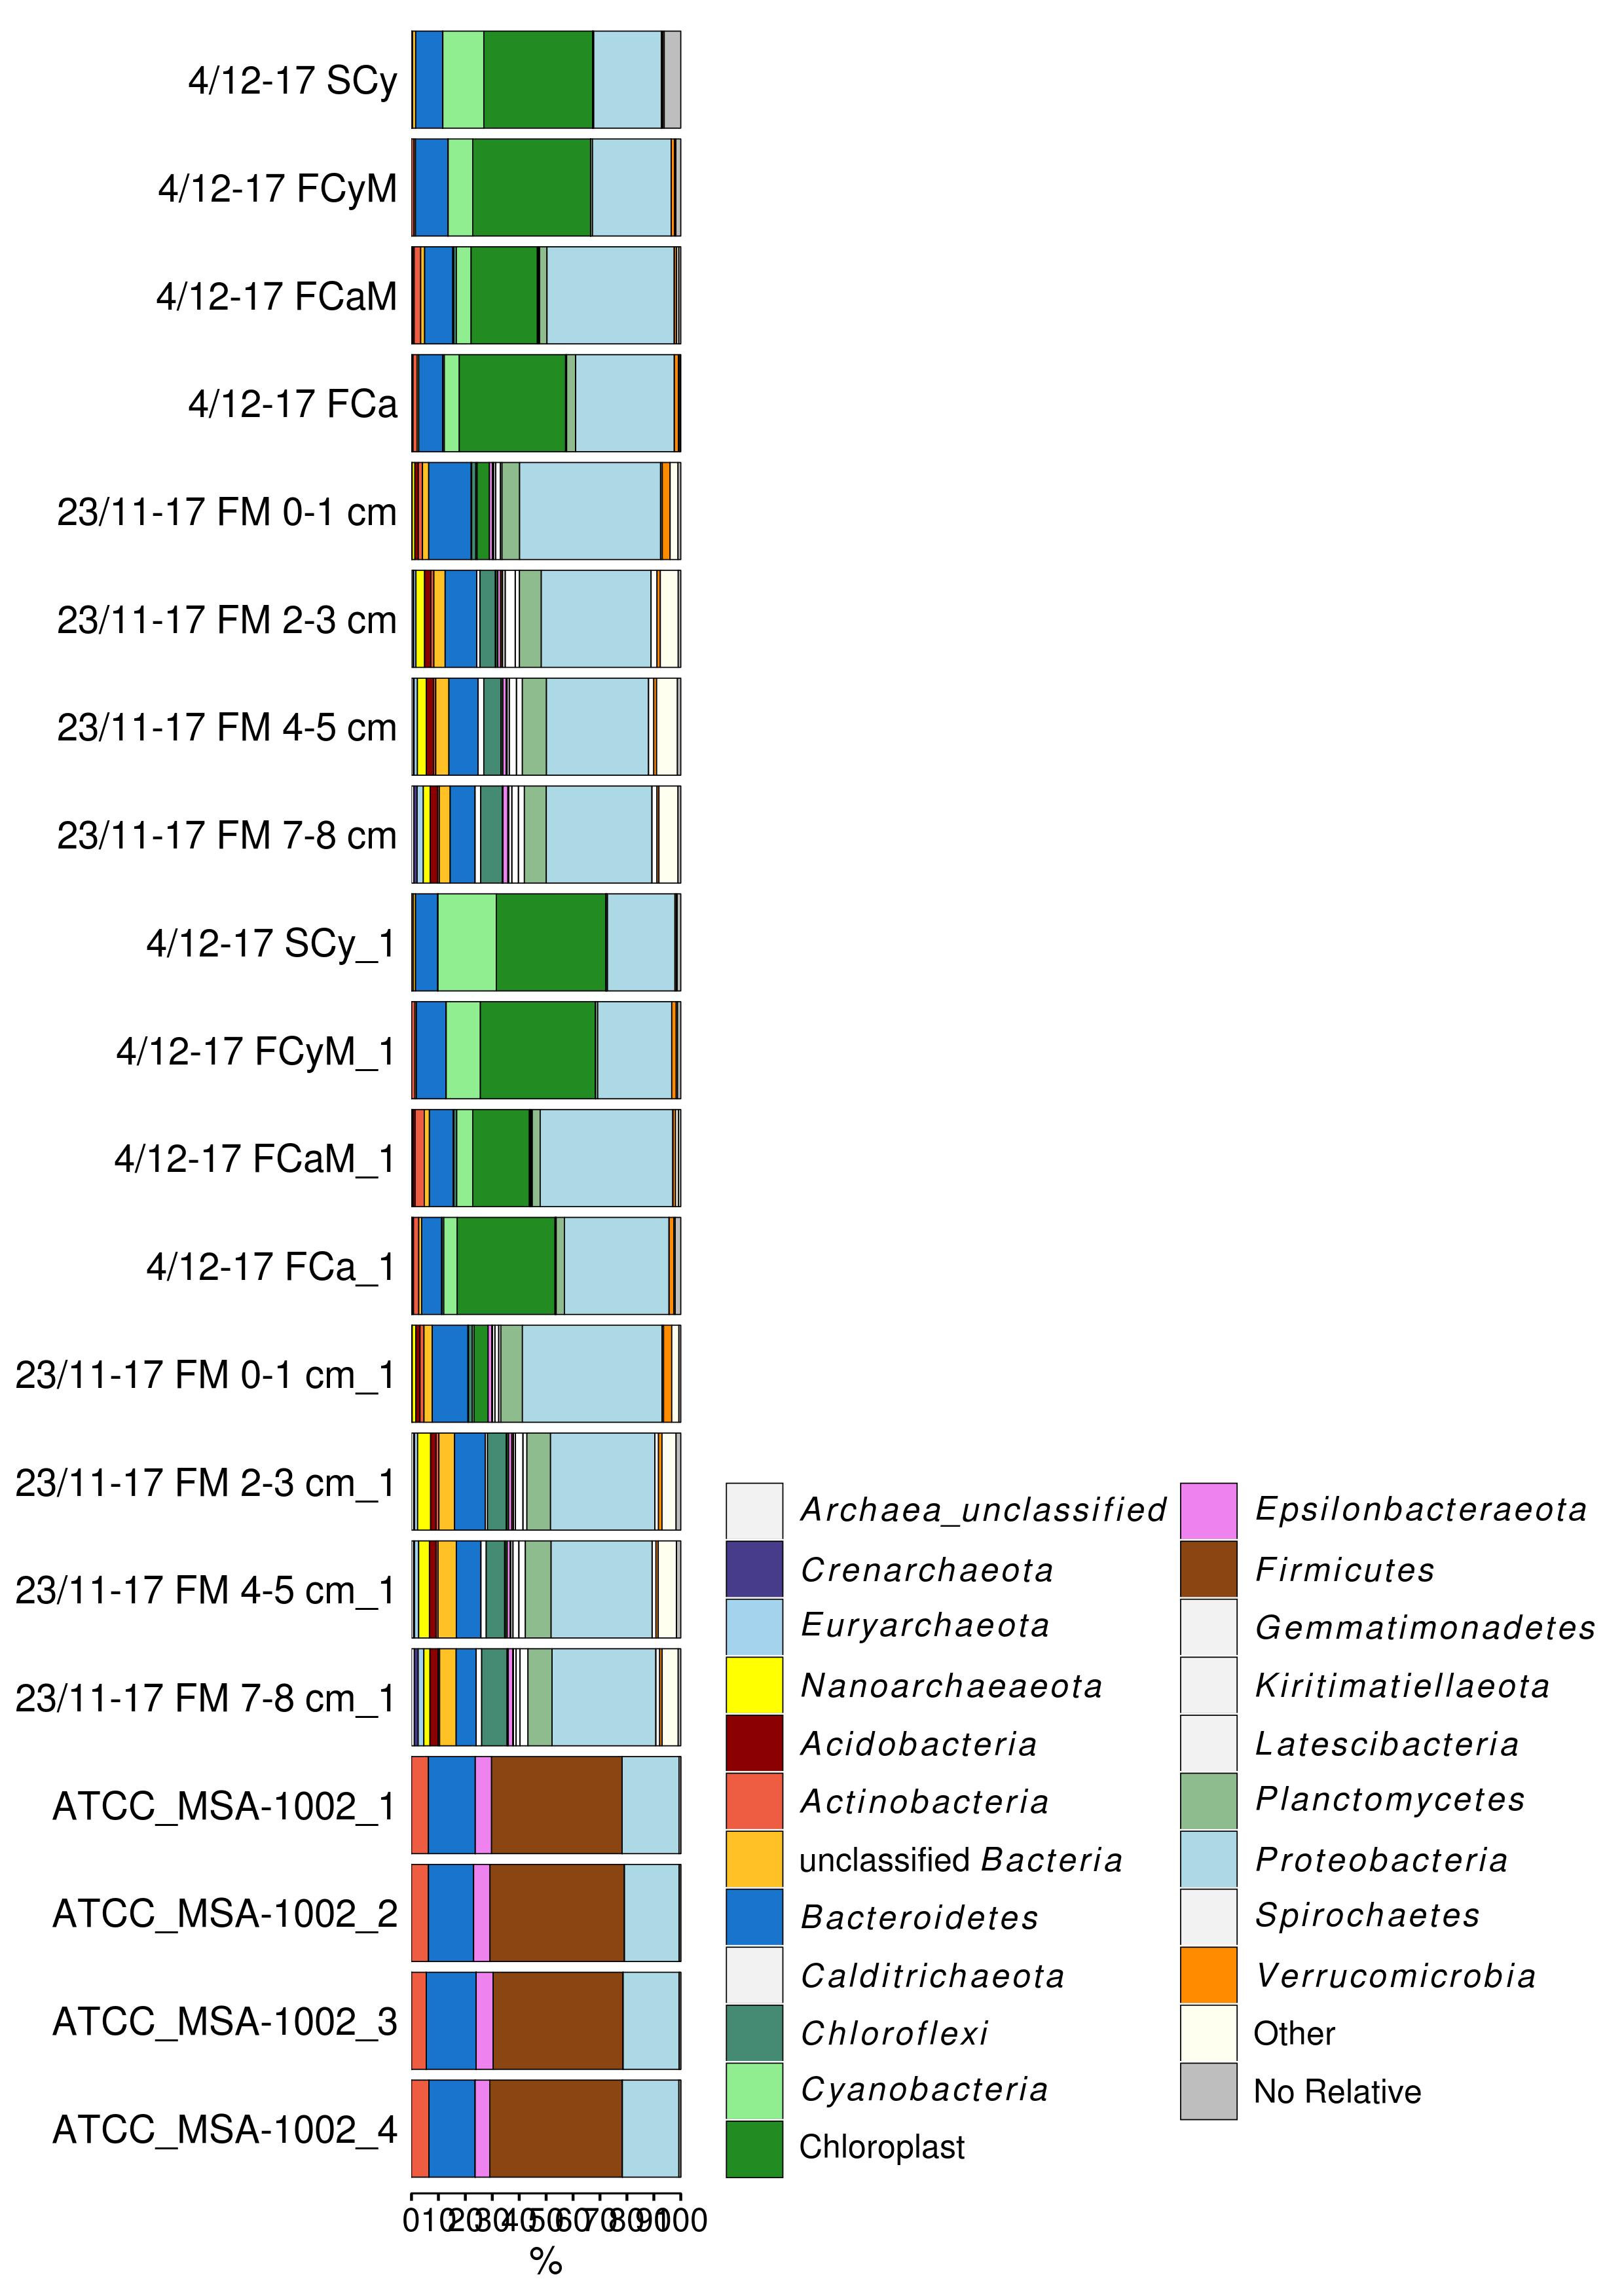
\includegraphics[width=1\linewidth]{../results/figures/community_barplot} 

}

\caption{Taxonomic classification and relative contribution of the most abundant bacterial sequences on the surfaces of two marine macrophytes (\textit{Cymodocea nodosa} and \textit{Caulerpa cylindracea}) from two locations (Saline and Funtana) and in two contrasting seasons (4 December 2017 and 19 June 2018).\label{community}}\label{fig:unnamed-chunk-2}
\end{figure}


\end{document}
